
% and then
% calculate the prediction $\lambda_{t+1} = \alpha + \beta (t+1)$. We can now
% compare $\lambda_{t+1}$ with the actual observation $y_{t+1}$. (Note: Care must
% be taken in the beginning as we need at least data for 3 years to make
% a fit of the line.) The mean squared prediction
% error is 1.5.

% Suppose that interest is also  in prediction  five
% years ahead. Then we can do as before and make predictions 
% $\lambda_{t+5} = \alpha + \beta (t+5)$. 
% Then we obtain the plot in Figure~\ref{fig:nht05}.
% The mean squared prediction
% error is 2.3.

% \begin{figure}[ht]
%   \centering
%   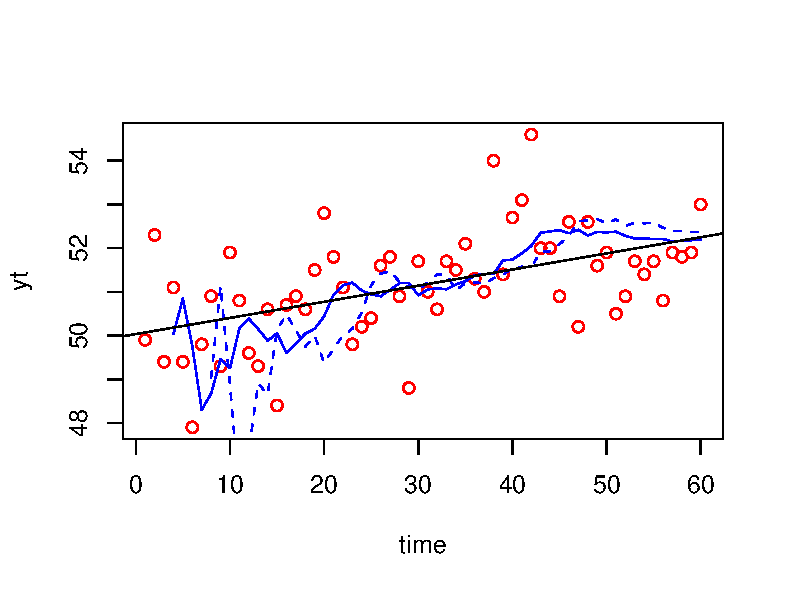
\includegraphics[height=6cm]{fig/nht-05}
%   \caption{New Hampshire temperatures and 1--step (solid line) and
%     5--step (dashed line) predictions based on
%     succesively fitting linear models to data. }
%   \label{fig:nht05}
% \end{figure}


\section{Dynamic linear models}
\label{sec:dlm}



An alternative is to think as follows: Instead of regarding
$(\alpha,\beta)$ as fixed but unknown parameters (who must then
necessarily remain unchanged over time), we allow $(\alpha,\beta)$ to
vary over time.  In particular the slope $\beta$
describes the rate of change in temperature and one could imagine that
this rate would vary (presumably slowly) over time. Hence we imagine that at time $t$
there is a specific value of the parameters $(\alpha_t, \beta_t)$
which we shall also write as $(\alpha,\beta)_t$. Hence we imagine that
$(\alpha,\beta)_t$ varies (slowly) over time. One way of achievieng
this is by postulating that 
\begin{equation}
  \label{eq:nht-syseq}
(\alpha,\beta)_t = (\alpha,\beta)_{t-1} + w_t  
\end{equation}
where $w_t \sim N_2(0,\Sigma_W)$ is a 2--dimensional error
term. 

To
make this work, we must know something about
$(\alpha,\beta)_{0}$, i.e.\ at time zero, i.e.\ before information
starts to arrive. A simple approach is to pick some (sensible)
starting values and write that 
$
(\alpha,\beta)_{0}= m_0 = (m_0^\alpha, m_0^\beta)=(50,0),
$ say. 
However, in practice there is a an uncertainty about
$(\alpha,\beta)_{0}$, so ysually, one would specify a distribution,
\begin{equation}
  \label{eq:nht-prior}
  (\alpha,\beta)_{0} \sim N_2(m_0, C_0)  
\end{equation}

Note two special cases: If $C_0=0$, then we are back to the simple
approach, of simply fixing $(\alpha,\beta)_{0}$ at a specified value. 
If $\Sigma_W=0$, then we are back to the original setting
where $(\alpha,\beta)_t$ is the same at all time points (almost, but
that is subtle little difference). 

The equations \eqref{eq:nht-obseq}, \eqref{eq:nht-syseq} and
\eqref{eq:nht-prior} all together specify a state space model as a
general term. A more specific term is a dynamic linear model (DLM)
because it is essentially a linear model with the additional twist
that the parameters are allowed to vary over time too.


\section{To be random or not to be random}

In a 'classical' regression setting as described in
Section~\ref{sec:nhtemp} the parameters $(\alpha,\beta)$ are regarded
as the true but unknown values. These are estimated, e.g.\ by least
squares regression. 

In Section~\ref{sec:dlm} the situation is different: Consider
\eqref{eq:nht-syseq}. Even if $(\alpha,\beta)_0$ is a fixed quantity,
then $(\alpha,\beta)_1$ will be a random variable because $w_1$ is a
random variable. A random variable is, by definition, random (!) so it
does not make sense to try to estimate it. Instead we estimate some
quantities which describes its distribution, and  a natural choice in
this connection could be the mean and variance. 










\section{Fitting the DLM}

We fit the DLM for the New Hampshire temperatures using the Kalman
filter. The 1--step and 5--step forecasts are displayed in
Figure~\ref{fig:nht06}. The mean squared prediction errors are
respectively 1.4 and 1.6. We have held the variance parameters fixed
at $\sigma^2_V=1$, $\sigma^2_W=\sigma^2_C=0.0001$. 
 
\begin{figure}[ht]
  \centering
  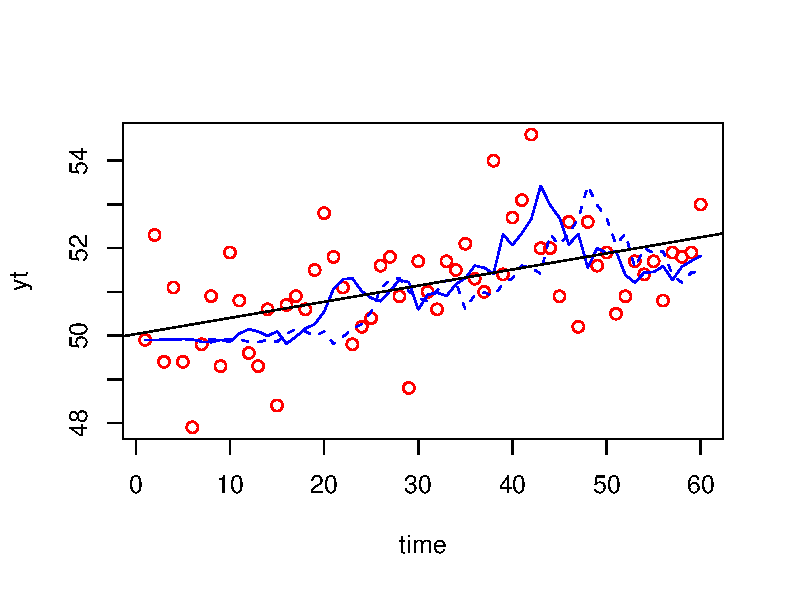
\includegraphics[height=6cm]{fig/nht-06}
  \caption{New Hampshire temperatures and 1--step (solid line) and
    5--step (dashed line) predictions based on fitting the DLM to  data. }
  \label{fig:nht06}
\end{figure}

The Kalman filter is very easy to implement in practice, see
Section~\ref{sec:KFimplement}. 

It is illustrative to look at e.g.\ the degree of smoothing for
different values of the variance parameters. In
Figure~\ref{fig:nht07}, we have fixed $\sigma^2_C=0.0001$ and vary 
$\sigma^2_V$ and $\sigma^2_W$. Smaller values of $\sigma^2_V$ and
larger values of $\sigma^2_W$ leads to
less smooth curves. 

\begin{figure}[ht]
  \centering
  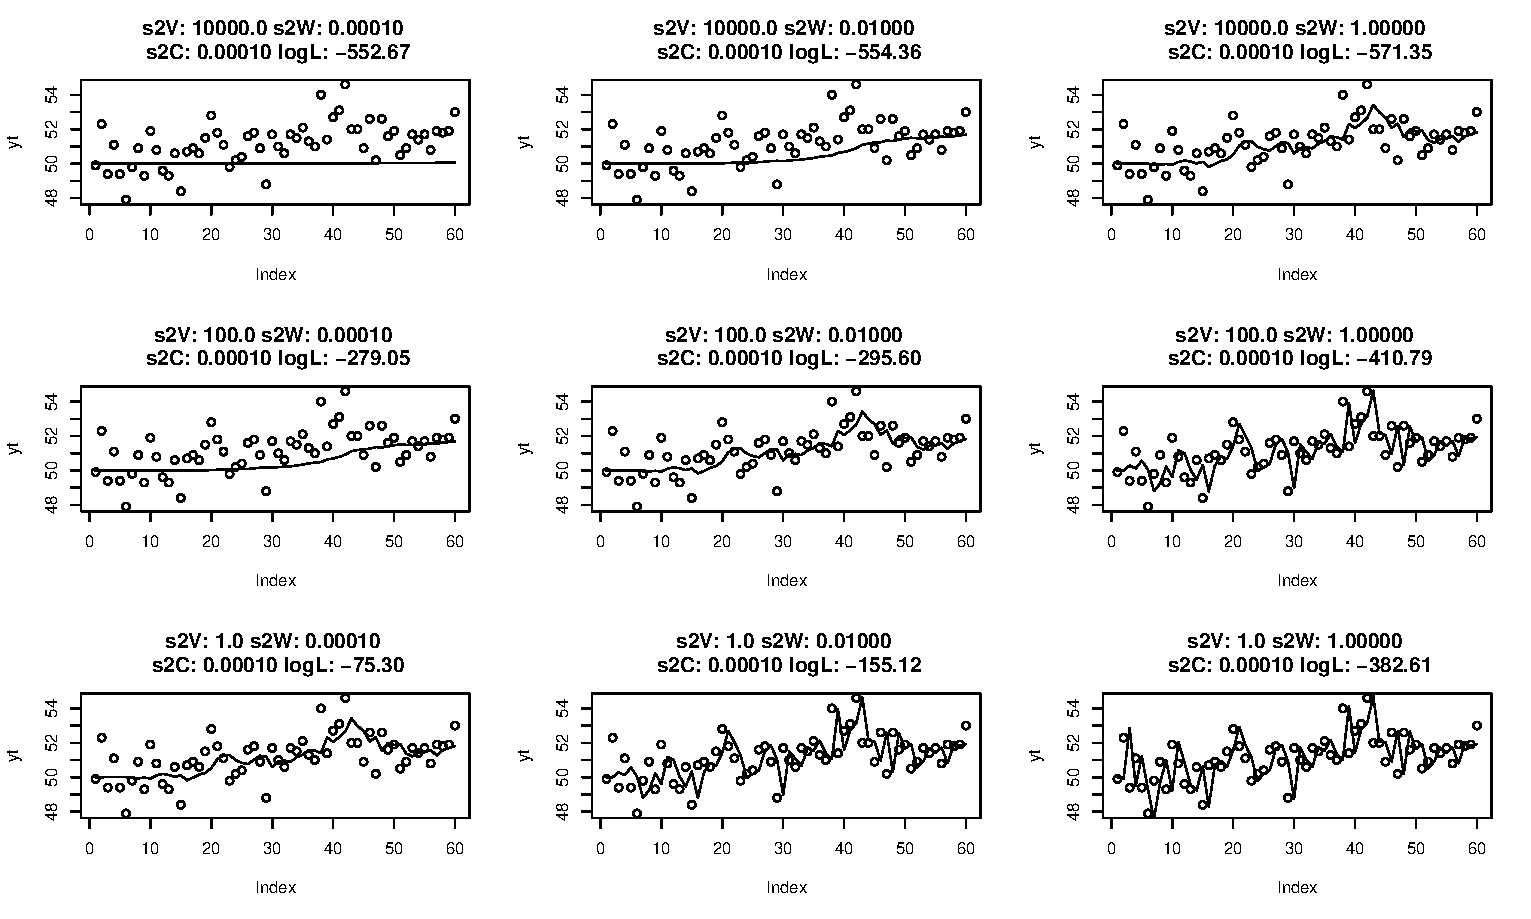
\includegraphics[height=9cm]{fig/nht-07}
  \caption{New Hampshire temperatures and 1--step  
    predictions based on fitting the DLM to data for different values
    of  $\sigma^2_V$ and $\sigma^2_W$. }
  \label{fig:nht07}
\end{figure}


\section{Another state space model}

Consider the model \eqref{eq:nht-obseq} again. If we let $E(y_t)=\mu_t=\alpha +
\beta t$ we get that $E(y_{t+1})= \mu_{t+1} = \mu_t + \beta$,
$E(y_{t+2})= \mu_{t+2} = \mu_t + 2\beta$ and so on. The stochastic
version of this is
\begin{eqnarray}
  y_t &=& \mu_t + v_t\\
  (\mu,\beta)_t &=& (\mu+\beta,\beta)_{t-1} + w_t
\end{eqnarray}



\begin{figure}[ht]
  \centering
  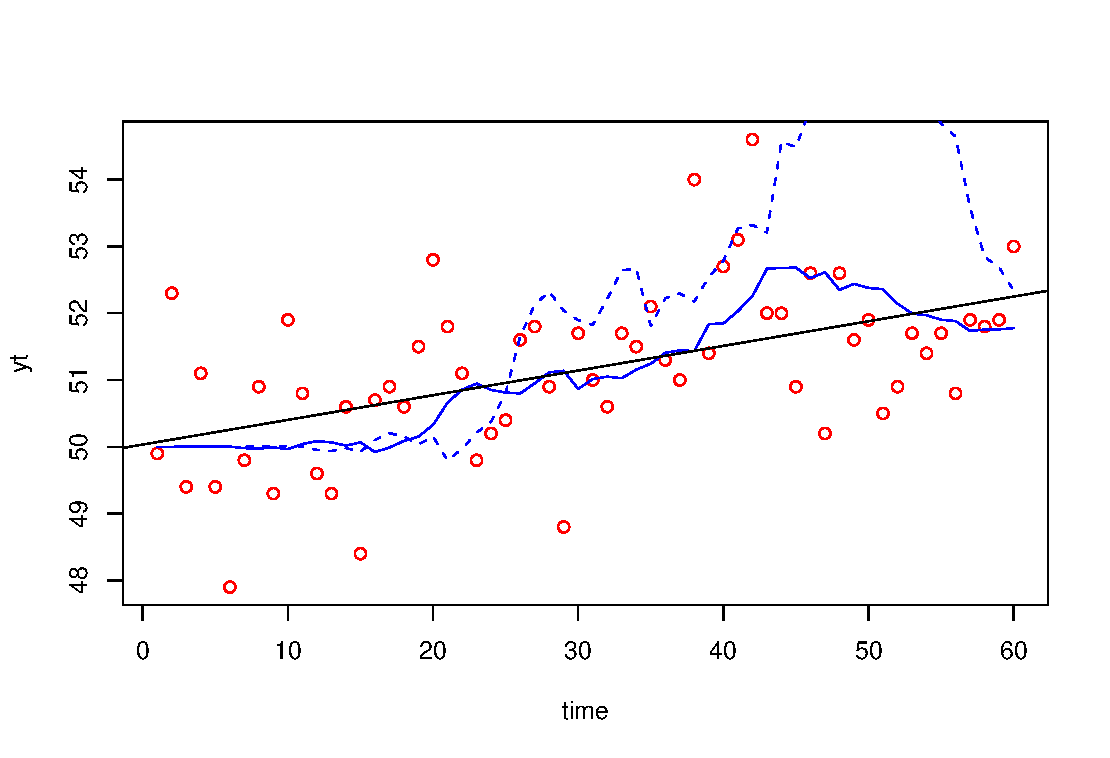
\includegraphics[height=6cm]{fig/nht-09}
  \caption{New Hampshire temperatures and 1--step  
    predictions based after ML estimation of $\sigma^2_V$ and
    $\sigma^2_W$ for three different values of $\sigma^2_C$. }
  \label{fig:nht09}
\end{figure}



Figure~\ref{fig:nht08} shows the result after fitting estimating 
 $\sigma^2_V$ and $\sigma^2_W$ for different values of
 $\sigma^2_C$. (It is in fact also possible to estimate $\sigma^2_C$
 but we abstain from this here). The influence of the prior variance
$\sigma^2_C$ is (not surprisingly) largest at the beginning of the
period.  

\begin{figure}[ht]
  \centering
  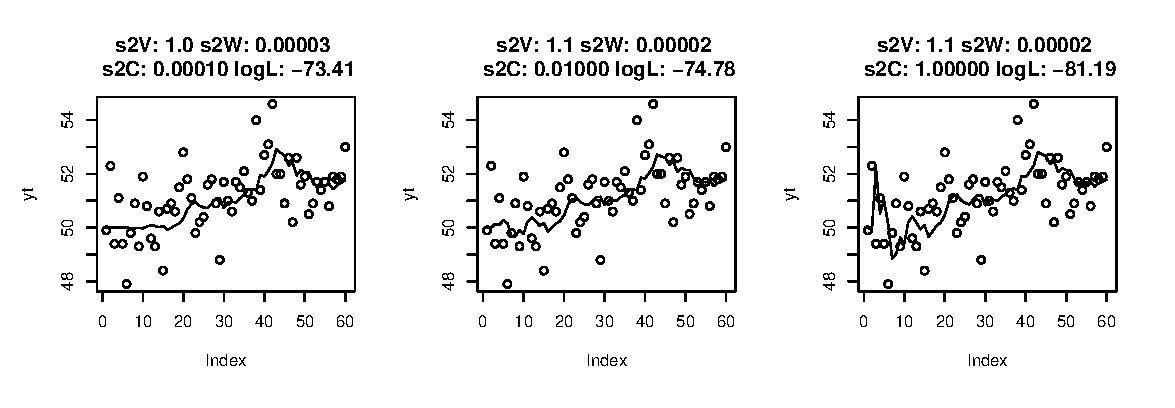
\includegraphics[width=13cm]{fig/nht-08}
  \caption{New Hampshire temperatures and 1--step  
    predictions based after ML estimation of $\sigma^2_V$ and
    $\sigma^2_W$ for three different values of $\sigma^2_C$. }
  \label{fig:nht08}
\end{figure}
